%-----------------------------------------------------------------------------%
\chapter{\babDua}
%-----------------------------------------------------------------------------%
Bagian ini berisi penjelasan mengenai teori-teori dan pengetahuan yang terkait dengan pelaksanaan penelitian.

%-----------------------------------------------------------------------------%
\section{Deep Learning}
%-----------------------------------------------------------------------------%
\textit{Deep Learning} merupakan teknik \textit{Machine Learning} yang menggunakan model \textit{Neural Network} yang terdiri dari beberapa lapisan pemrosesan untuk melakukan klasifikasi. Teknik \textit{Machine Learning} konvensional memerlukan representasi data (fitur-fitur data) sebagai masukan untuk melakukan klasifikasi. Pada \textit{Deep Learning}, model dapat menerima masukan berupa data mentah. Model dapat secara otomatis mempelajari dan menghasilkan representasi data yang diperlukan untuk melakukan klasifikasi. Oleh karena itu \textit{Deep Learning} merupakan salah satu bentuk dari \textit{Representation Learning}. Pada suatu model \textit{Deep Learning} terdapat lapisan-lapisan yang bertugas untuk mempelajari dan menghasilkan representasi data dan terdapat lapisan-lapisan yang bertugas untuk melakukan klasifikasi \cite{deeplearning}. 

Contoh model \textit{Deep Learning} yang populer adalah \textit{Convolutional Neural Network} (CNN). CNN dapat memproses data berupa citra, video, maupun audio. CNN tersusun dari beberapa lapisan pemrosesan yang masing-masing terdiri dari beberapa \textit{node}. Pada bagian awal model terdapat lapisan konvolusi yang berfungsi untuk menghasilkan fitur-fitur dari data dengan cara melakukan konvolusi menggunakan suatu filter. Lapisan konvolusi dapat disambungkan dengan lapisan \textit{pooling} yang berfungsi untuk melakukan \textit{downsampling} terhadap data. Pada bagian akhir model biasanya terdapat lapisan \textit{fully-connected}, lapisan yang setiap \textit{node}-nya terhubung dengan setiap \textit{node} pada lapisan tetangganya. Lapisan ini bertugas untuk melakukan klasifikasi menggunakan fitur-fitur data yang diperoleh dari lapisan-lapisan sebelumnya \cite{deeplearning}. \pic~\ref{fig:cnn} merupakan contoh model CNN.

\begin{figure}
	\centering
	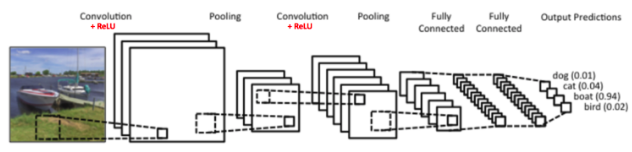
\includegraphics[width=0.75\textwidth]
	{pics/cnn.png}
	\caption{Contoh model \textit{Convolutional Neural Network} yang mengandung lapisan konvolusi, lapisan \textit{pooling}, dan lapisan \textit{fully-connected}.}
	\label{fig:cnn}
\end{figure}

%-----------------------------------------------------------------------------%
\section{Proses Latihan dan \textit{Inference} pada Deep Learning}
%-----------------------------------------------------------------------------%
Lapisan-lapisan pada model \textit{Deep Learning} memiliki suatu parameter yang digunakan untuk menghitung nilai dari masing-masing \textit{node} pada lapisan. Nilai dari parameter tersebut dapat diatur melalui proses latihan. Proses latihan bertujuan untuk memperbarui nilai parameter pada setiap lapisan dengan harapan akurasi model dalam melakukan klasifikasi akan meningkat. Salah satu metode latihan adalah dengan menggunakan sekumpulan data yang telah diketahui labelnya (\textit{Supervised Learning}). Model melakukan prediksi terhadap label dari data-data tersebut dengan melakukan \textit{forward propagation}. Label hasil prediksi kemudian dibandingkan dengan label asli yang telah diketahui. Informasi galat dari hasil prediksi kemudian dikirimkan ke semua lapisan, mulai dari lapisan paling akhir hingga lapisan paling awal (\textit{backward propagation}). Galat tersebut digunakan untuk memperbarui nilai parameter pada setiap lapisan dengan tujuan untuk mengurangi galat pada prediksi-prediksi selanjutnya \cite{deeplearning}. 

Proses \textit{inference} sedikit berbeda dengan proses latihan. Proses \textit{inference} bertujuan untuk memprediksi label dari suatu data (pada umumnya data baru yang belum diketahui labelnya) tanpa melakukan pembaruan nilai parameter. Pada proses ini hanya terjadi \textit{forward-propagation}. Komputasi dilakukan terhadap data mulai dari lapisan pertama, kemudian diteruskan ke lapisan kedua, dan seterusnya hingga mencapai lapisan terakhir. Data pada lapisan terakhir adalah hasil dari \textit{forward-propagation} yang selanjutnya digunakan untuk menentukan label atau kelas dari data \cite{trainvsinfer}. \pic~\ref{fig:cnn} menunjukkan perbedaan proses latihan dan \textit{inference}.

\begin{figure}
	\centering
	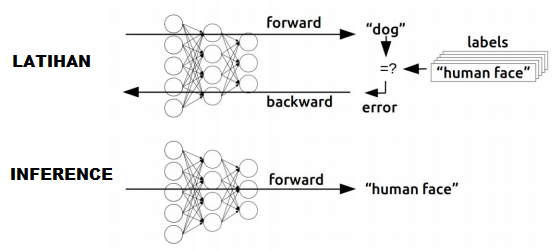
\includegraphics[width=0.75\textwidth]
	{pics/trainingvsinference.png}
	\caption{Perbedaan proses latihan dan \textit{inference} pada \textit{Deep Learning}.}
	\label{fig:trainvsinfer}
\end{figure}

\section{Operasi-operasi Deep Learning Inference}
%-----------------------------------------------------------------------------%
Proses \textit{inference} pada \textit{Deep Learning} melibatakan beberapa operasi matriks yang cukup berat, dua di antaranya adalah operasi konvolusi matriks dan operasi perkalian matriks-matriks. Dua operasi inilah yang pada penelitian ini akan diimplementasikan menggunakan OpenCL dan dijalankan di \textit{mobile} GPU.

\subsection{Konvolusi Matriks}
Operasi konvolusi matriks terjadi pada lapisan konvolusi. Operasi ini melibatkan tiga buah matriks yaitu matriks masukan, matriks filter, dan matriks keluaran. Matriks-matriks tersebut memiliki tiga dimensi yaitu kanal, baris, dan kolom. Banyaknya kanal menyatakan kedalaman matriks, banyaknya baris menyatakan ketinggian matriks, dan banyaknya kolom menyatakan lebar matriks.

Pada lapisan konvolusi, terjadi operasi konvolusi antara matriks filter dan matriks masukan. Suatu matriks masukan dapat dikonvolusikan dengan satu atau lebih filter. Karena itu, filter juga dapat dipandang sebagai matriks yang memiliki empat dimensi yaitu kanal, baris, kolom, dan \textit{batch}. Banyaknya \textit{batch} menyatakan banyaknya filter tiga dimensi (kanal, baris, dan kolom). Konvolusi dari satu \textit{batch} pada filter menghasilkan satu kanal tersendiri pada matriks keluaran, sehingga banyaknya \textit{batch} pada filter akan selalu sama dengan banyaknya kanal (kedalaman) dari matriks keluaran.	

Pada operasi konvolusi, posisi filter dimulai dari ujung kiri atas dari matriks masukan. Filter kemudian bergeser ke kanan dan kebawah dengan besar jangkah yang ditentukan (pada umumnya besarnya jangkah adalah satu). Pada suatu posisi filter, dilakukan perkalian titik antara matriks filter dengan submatriks dari matriks masukan yang bersesuaian dengan posisi filter. Karena terjadi perkalian titik, maka kedalaman matriks masukan pasti selalu sama dengan kedalaman matriks filter. Satu kali operasi perkalian titik tersebut menghasilkan skalar yang merupakan satu elemen dari matriks keluaran. Setelah proses konvolusi selesai untuk satu \textit{batch} filter, akan terbentuk satu kanal pada matriks keluaran \cite{deeplearningmatrix}. \pic~\ref{fig:conv} menunjukkan contoh operasi konvolusi dengan matriks masukan berukuran $5 \times 5$ (satu kanal), filter berukuran $3 \times 3$ (satu kanal dan satu \textit{batch}), dan jangkah sebesar satu.

\begin{figure}
	\centering
	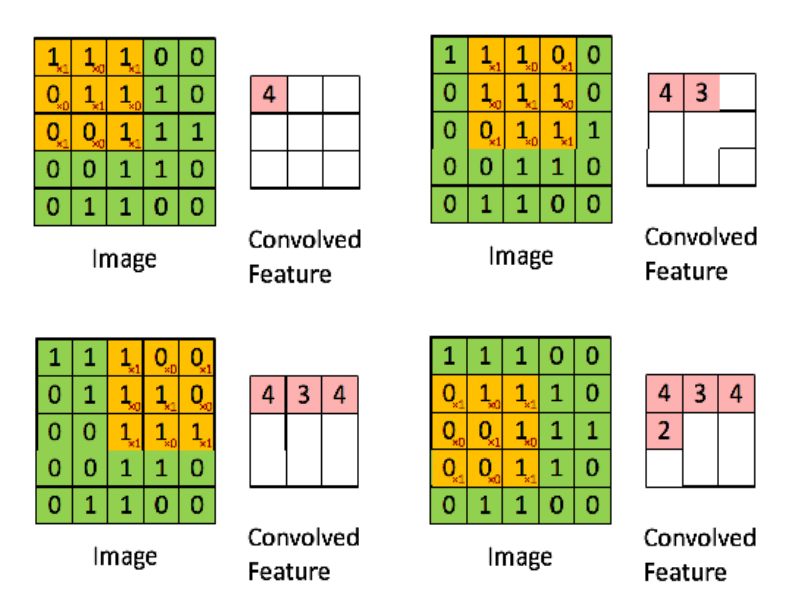
\includegraphics[width=0.75\textwidth]
	{pics/conv.png}
	\caption{Contoh operasi konvolusi.}
	\label{fig:conv}
\end{figure}

Suatu operasi konvolusi dapat dilakukan sekaligus terhadap lebih dari satu matriks masukan dan menghasilkan lebih dari satu matriks keluaran. Jika demikian, maka matriks masukan dan matriks keluaran juga dapat dianggap sebagai matriks yang memiliki empat dimensi seperti matriks filter dengan dimensi tambahan yaitu \textit{batch}.

\subsection{Perkalian Matriks-Matriks}
Operasi perkalian matriks-matriks pada \textit{Deep Learning inference} terjadi pada lapisan \textit{fully-connected}. Pada lapisan ke-\textit{l} dari model, nilai parameter disimpan dalam bentuk matriks dua dimensi berukuran $M \times K$, dimana $M$ adalah banyaknya \textit{node} pada lapisan ke-\textit{l} dan $K$ adalah banyaknya \textit{node} pada lapisan ke-\textit{(l-1)}. Baris ke-\textit{i} dari matriks parameter pada lapisan ke-\textit{l} tersebut merupakan vektor parameter untuk \textit{node} ke-\textit{i} pada lapisan ke-\textit{l}. Untuk memperoleh nilai semua \textit{node} pada lapisan ke-\textit{l}, matriks parameter dikalikan dengan vektor sepanjang $K$ yang elemen-elemennya adalah nilai-nilai \textit{node} pada lapisan ke-\textit{(l-1)}. Hasilnya adalah vektor sepanjang $M$, sesuai dengan banyaknya \textit{node} pada lapisan ke-\textit{l} \cite{deeplearningmatrix}. \pic~\ref{fig:fcmatmul} menunjukkan bagaimana operasi perkalian matriks-vektor ini terjadi. 

\begin{figure}
	\centering
	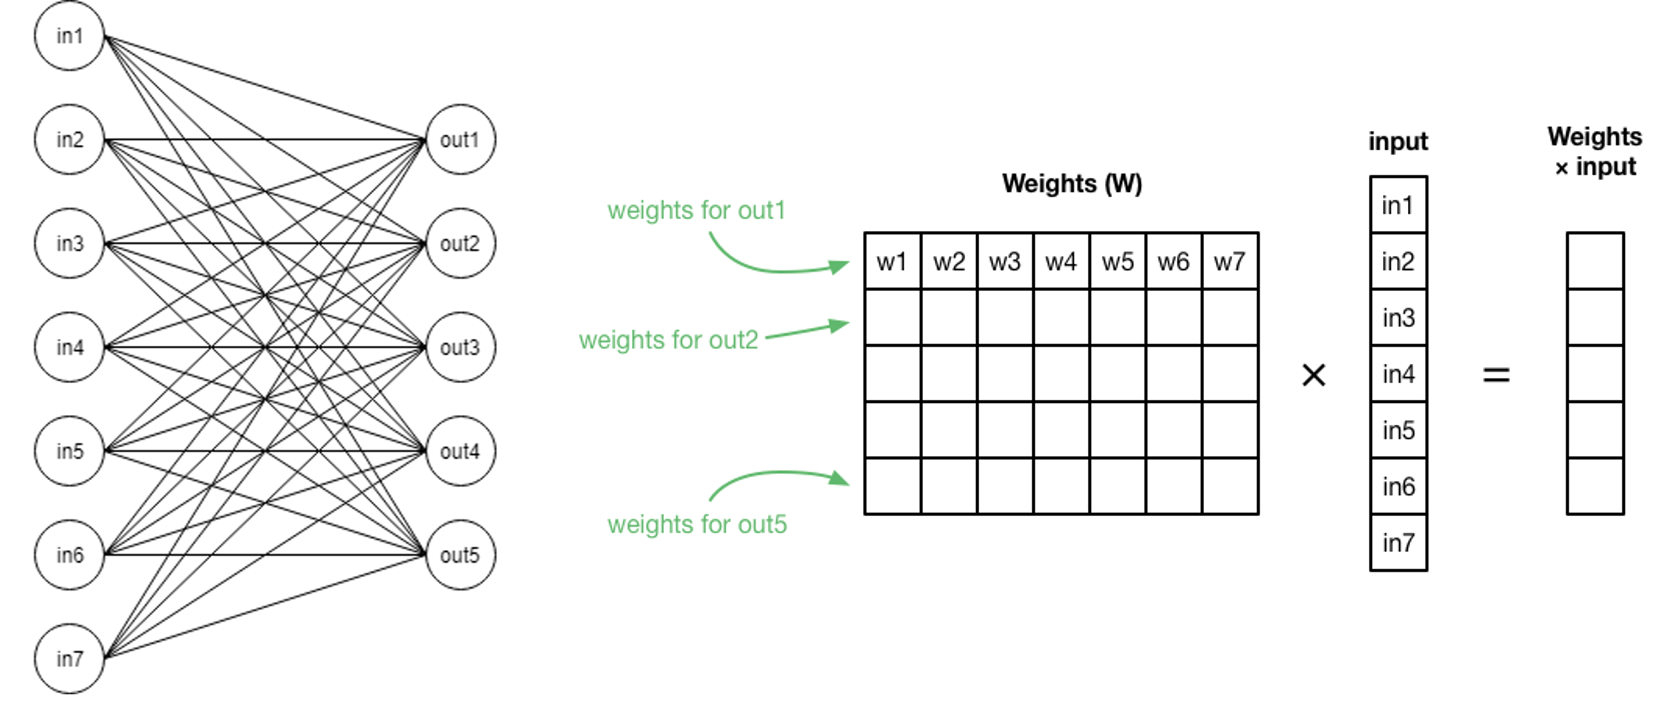
\includegraphics[width=0.75\textwidth]
	{pics/fcmatmul.png}
	\caption{Ilustrasi perkalian matriks-vektor pada lapisan \textit{fully-connected}, dimana elemen ke-$i$ pada vektor $weight \times input$ adalah nilai $out_i$.}
	\label{fig:fcmatmul}
\end{figure}

Operasi perkalian matriks berukuran $M \times K$ dengan vektor berukuran $K \times 1$ pada lapisan \textit{fully-connected} tersebut dapat dilakukan sekaligus untuk $N$ \textit{batch}, sehingga akan terjadi operasi perkalian matriks-matriks antara matriks berukuran $M \times K$ dengan matriks berukuran $K \times N$ yang menghasilkan matriks berukuran $M \times N$.

Selain lapisan \textit{fully-connected}, operasi perkalian matriks-matriks juga dapat terjadi pada lapisan konvolusi, yaitu ketika operasi konvolusi melibatkan filter yang berukuran $tinggi \times lebar = 1 \times 1$. Matriks masukan dari operasi konvolusi dapat dipandang sebagai matriks dua dimensi dengan tinggi $H_{i} \times W_{i} \times B_{i}$ dan lebar $C_{i}$ dimana $H_{i}$, $W_{i}$, $C_{i}$, dan $B_{i}$ berturut-turut adalah tinggi, lebar, banyaknya kanal, dan banyaknya \textit{batch} dari matriks masukan. Sementara itu filter dapat dipandang sebagai matriks dua dimensi dengan tinggi $C_{f}$ dan lebar $H_{f} \times W_{f} \times B_{f}$ dimana $H_{f}$, $W_{f}$, $C_{f}$, dan $B_{f}$ berturut-turut adalah tinggi, lebar, banyaknya kanal, dan banyaknya \textit{batch} dari matriks filter.

\section{Tensorflow Lite}
%-----------------------------------------------------------------------------%
TensorFlow \cite{tensorflow} adalah perangkat lunak sumber terbuka yang merupakan pustaka untuk melakukan komputasi numerik menggunakan graf. \textit{Node} pada graf merepresentasikan operasi matematika, sedangkan \textit{edge} pada graf merepresentasikan \textit{tensor} (larik multidimensi) sebagai masukan atau keluaran dari operasi pada \textit{node}. Tensorflow dikembangkan oleh para pengembang dan peneliti dari Google untuk keperluan penelitian di bidang \textit{Machine Learning} and \textit{Deep Learning}. Selain dapat digunakan pada komputer personal atau \textit{server}, Tensorflow juga digunakan pada perangkat \textit{mobile} untuk menjalankan proses \textit{inference} melalui pustaka Tensorflow Lite.

Tensorflow Lite \cite{tflite} merupakan pustaka \textit{Machine Learning} terbaru dari Tensorflow yang ditujukan untuk perangkat Android dan IoS. Tensorflow Lite diimplementasikan menggunakan bahasa C/C++. Saat ini Tensorflow Lite memiliki dukungan untuk menjalankan proses \textit{inference} pada model CNN dan LSTM. Tensorflow Lite memiliki \textit{kernel} tersendiri yang terpisah dari pusat Tensorflow. Yang dimaksud dengan \textit{kernel} pada Tensorflow Lite adalah program yang digunakan untuk menjalankan proses \textit{inference} pada \textit{Deep Learning}. Contoh \textit{kernel} pada Tensorflow Lite adalah \textit{kernel} perkalian matriks-matriks dan \textit{kernel} konvolusi matriks. Tensorflow Lite memiliki suatu jenis \textit{kernel} yang telah dioptimalkan untuk perangkat \textit{mobile}, yaitu \textit{optimized kernel}, yang memiliki performa yang sangat baik. Selain \textit{optimized kernel} terdapat pula jenis \textit{kernel} biasa, yaitu \textit{naive kernel}, yang performanya tidak lebih baik dari \textit{optimized kernel}.

Untuk melakukan proses \textit{inference}, Tensorflow Lite memerlukan graf dengan format ".tflite" yang berisi model \textit{Deep Learning}. Graf tersebut akan diinterpretasi oleh \textit{interpreter} pada Tensorflow Lite. \textit{Interpreter} akan memuat semua \textit{kernel} yang diperlukan oleh model pada graf tersebut secara selektif. \pic~\ref{fig:tflite} menunjukkan arsitektur Tensorfow Lite.

\begin{figure}
	\centering
	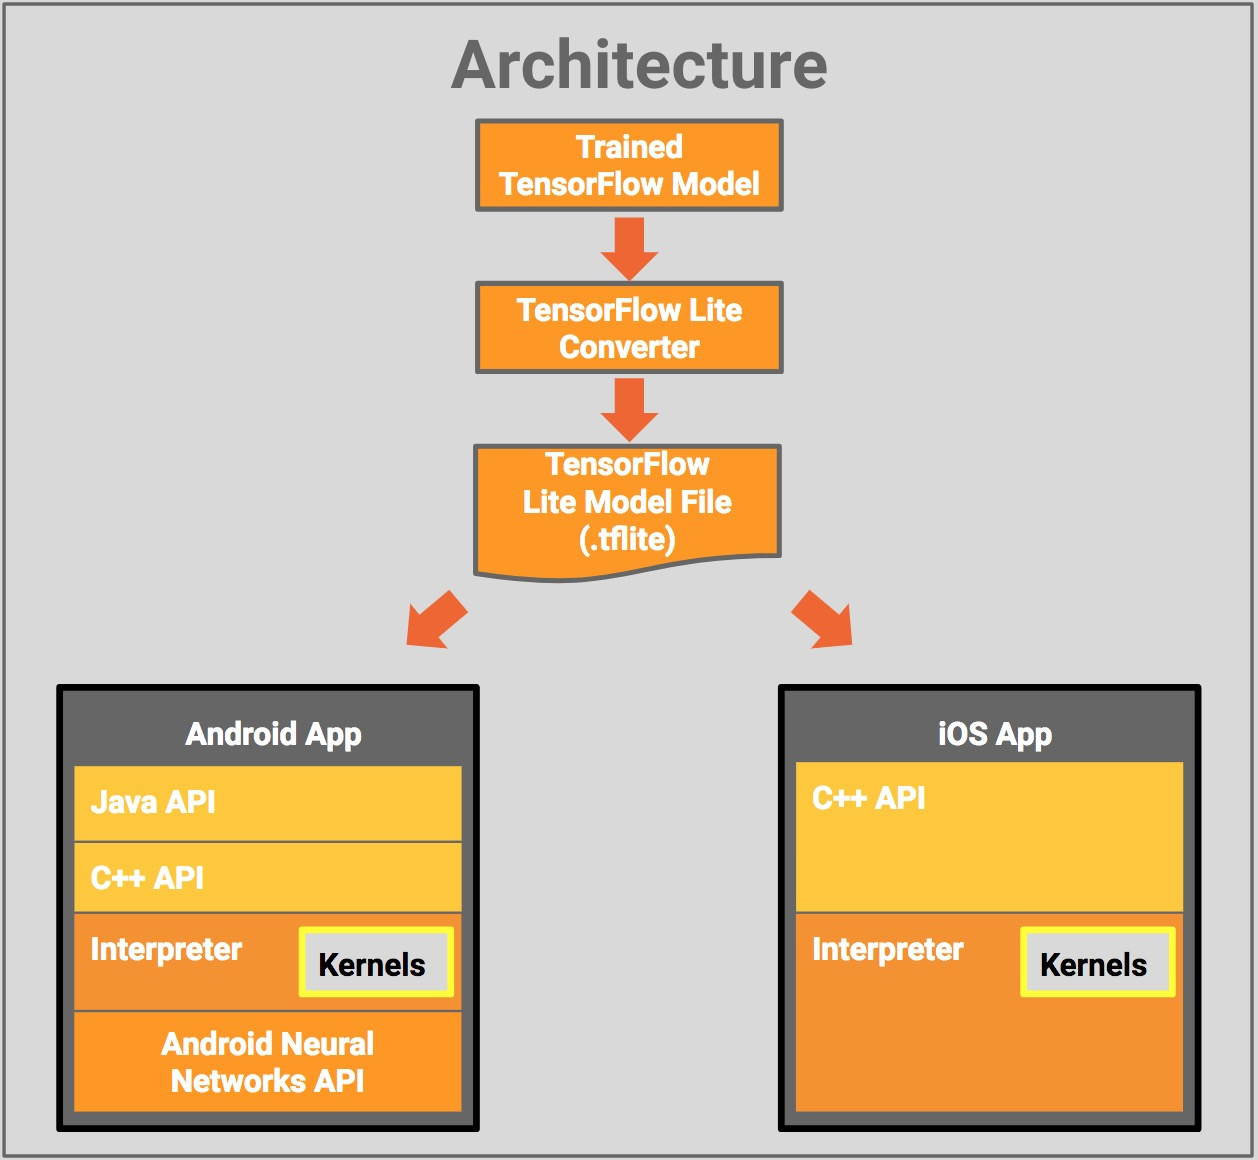
\includegraphics[width=0.75\textwidth]
	{pics/tflite.jpg}
	\caption{Arsitektur Tensorflow Lite dengan \textit{interpreter} yang bertugas memuat \textit{kernel} yang diperlukan secara selektif.}
	\label{fig:tflite}
\end{figure}

\section{OpenCL}
%-----------------------------------------------------------------------------%
OpenCL merupakan API untuk melakukan pemrograman paralel pada prosesor yang berbeda-beda seperti CPU, GPU, dan FPGA. OpenCL dapat digunakan untuk meningkatkan performa komputasi secara signifikan. OpenCL API tersedia dalam bahasa C/C++ dengan ekstensi. Pada OpenCL terdapat dua sisi program, yaitu \textit{host} dan \textit{device}. \textit{Device} adalah prosesor target tempat berjalannya komputasi. \textit{Host} adalah yang mengatur jalannya komputasi pada \textit{device}. Menyalin data masukan dari memori \textit{host} ke memori \textit{device} dan menentukan banyaknya \textit{thread} yang bekerja adalah contoh tugas dari \textit{host}. OpenCL \textit{device} pada penelitian ini adalah GPU. Dalam suatu program OpenCL terdapat istilah-istilah yang perlu dipahami sebagai berikut \cite{openclguide}.

\begin{enumerate}
	\item \textbf{\textit{Kernel}}. \textit{Kernel} pada OpenCL adalah serangkaian instruksi yang mendefinisikan suatu fungsi tertentu, sama seperti fungsi pada C/C++. \textit{Kernel} dieksekusi pada \textit{device}, namun dikompilasi dan dijadwalkan eksekusinya oleh \textit{host}.
	
	\item \textbf{\textit{Buffer}}. \textit{Buffer} merupakan objek memori yang menyimpan koleksi data secara linear dalam \textit{bytes}. \textit{Buffer} berada pada memori \textit{device} (dalam penelitian ini adalah memori GPU). OpenCL \textit{kernel} dapat mengakses data pada \textit{buffer} menggunakan \textit{pointer} yang diberikan melalui argumen \textit{kernel}. Data pada \textit{buffer} juga dapat dimanipulasi oleh \textit{host}.
	
	\item \textbf{\textit{Command Queue}}. \textit{Command queue} merupakan objek yang menampung perintah-perintah yang akan dieksekusi pada \textit{device}. OpenCL \textit{kernel} dijadwalkan eksekusinya melalui \textit{command queue}.
	
	\item \textbf{\textit{Context}}. \textit{Context} adalah lingkungan dimana komputasi pada \textit{device} dilakukan. Pada \textit{context} didefiniskan \textit{kernel} yang digunakan, \textit{device} yang digunakan, \textit{buffer} yang dapat diakses oleh \textit{kernel}, dan \textit{command queue} yang digunakan.
	
\end{enumerate}

Tahap-tahap berjalannya suatu program OpenCL dapat dilihat pada \tab~\ref{tab:OpenCLexecutionorder}. Sebelum suatu OpenCL \textit{kernel} dapat dieksekusi pada \textit{device}, \textit{host} perlu melakukan beberapa persiapan seperti pada \tab~\ref{tab:OpenCLexecutionorder}. Ketika persiapan telah selesai, OpenCL \textit{kernel} dapat dijadwalkan eksekusinya dengan cara melakukan \textit{enqueue} terhadap \textit{command queue}. Data-data yang terkait dengan eksekusi OpenCL \textit{kernel} (misalnya matriks masukan dan matriks keluaran) perlu disalin secara manual dari memori \textit{host} ke memori \textit{device} dan sebaliknya.

\begin{table}
	\centering
	\caption{Tahap-tahap eksekusi program OpenCL dari awal hingga akhir.}
	\label{tab:OpenCLexecutionorder}
	\begin{tabular}{| >{\small}l | >{\small}l |}
		\hline
		\textbf{No.} & \textbf{Tahap}\\ 
		\hline
		1 & Membuat \textit{context} \\ 
		\hline 
		2 & Membuat \textit{kernel}\\ 
		\hline 
		3 & Membuat \textit{comand-queue}\\ 
		\hline
		4 & Membuat \textit{buffer}\\ 
		\hline
		5 & Menyalin data masukan dari \textit{host memory} ke \textit{device memory}.\\
		\hline
		6 & Mendefinisikan struktur \textit{work-space}.\\
		\hline
		7 & Mendefinisikan argumen-argumen \textit{kernel}.\\
		\hline
		8 & Eksekusi \textit{kernel}. \\
		\hline
		9 & Menyalin data keluaran dari 
		\textit{device memory} ke \textit{host memory}. \\
		\hline
	\end{tabular}
\end{table}				

Untuk mengimplementasikan OpenCL, diperlukan pustaka OpenCL ("libOpenCL.so") dan OpenCL \textit{headers} ("cl.h" dan "cl\_platform.h"). Pada NVIDIA GPU, pustaka OpenCL dapat diperoleh dalam paket instalasi CUDA. Pada perangkat Android, pustaka OpenCL disediakan oleh vendor dari masing-masing prosesor. Perangkat Android dengan vendor GPU Adreno atau Mali biasanya sudah dilengkapi dengan pustaka OpenCL yang terletak pada direktori "/system/vendor/lib/". Pustaka tersebut dapat diambil menggunakan perintah "adb pull" pada Linux.

\section{Paralelisasi pada OpenCL}
%-----------------------------------------------------------------------------%
\textit{Kernel} pada OpenCL dapat dijalakan oleh banyak \textit{thread}. Semua \textit{thread} menjalakan \textit{kernel} yang sama, namun dapat dibuat sedemikian sehingga bagian data yang diproses oleh setiap \textit{thread} berbeda. Ini adalah teknik pemrograman paralel yang umum digunakan pada OpenCL. Misalnya operasi penjumlahan dua buah vektor sepanjang $N$ dapat dikerjakan oleh $N$ \textit{thread}, dimana \textit{thread} ke-\textit{i} hanya menjumlahkan elemen ke-\textit{i} dari dua vektor tersebut. Pada OpenCL, \textit{thread} ini disebut \textit{work-item}. Seluruh \textit{work-item} yang mengeksekusi suatu \textit{kernel} membentuk blok dalam suatu ruang $N$ dimensi yang disebut \textit{NDRange}. Nilai $N$ yang valid hingga saat ini adalah 1, 2, dan 3. Semua \textit{work-item} pada suatu \textit{NDRange} dikelompokkan ke dalam \textit{work-group}. \textit{Work-group} terdiri dari beberapa \textit{work-item} yang membentuk blok satu hingga tiga dimensi \cite{openclguide}.

Setiap \textit{work-item} memiliki pengidentifikasi (ID) yang unik. ID adalah bilangan bulat yang lebih besar dari atau sama dengan nol. Setiap \textit{work-item} memiliki dua jenis ID, yaitu ID global dan ID lokal. ID global mengidentifikasi \textit{work-item} dalam suatu \textit{NDRange}, sedangkan ID lokal mengidentifikasi \textit{work-item} dalam suatu \textit{work-group}. Setiap \textit{work-group} juga memiliki ID yang unik. Saat suatu proses berjalan pada \textit{device}, ID dari \textit{work-item} dan \textit{work-group} yang menjalankan proses tersebut dapat diambil dan dapat dimanfaatkan untuk mengatur paralelisasi dari eksekusi OpenCL \textit{kernel} \cite{opencl}. \pic~\ref{fig:work} adalah contoh \textit{NDRange} dua dimensi pada OpenCL.

\begin{figure}
	\centering
	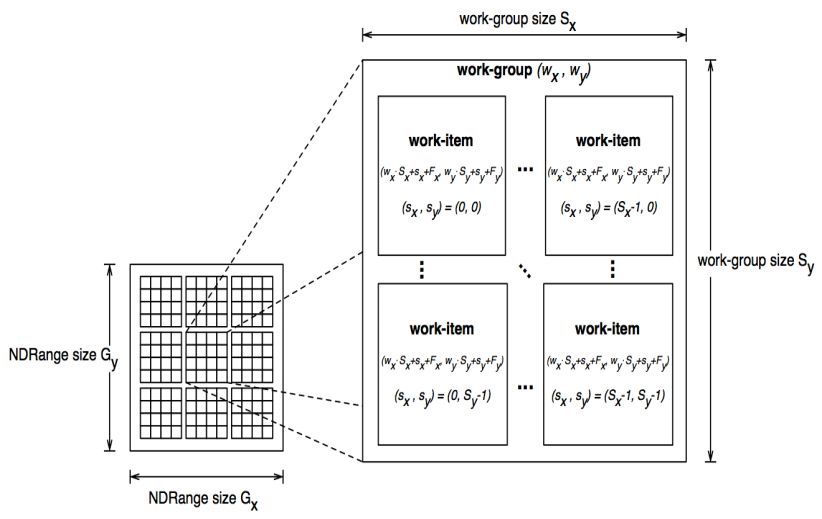
\includegraphics[width=0.75\textwidth]
	{pics/opencl-work.png}
	\caption{Contoh \textit{NDRange} dua dimensi yang terdiri dari beberapa \textit{work-group} dua dimensi.}
	\label{fig:work}
\end{figure}

Pada GPU, semua \textit{work-item} dalam suatu \textit{work-group} bekerja secara konkuren pada suatu unit komputasi. Sinkronisasi dapat dilakukan antara semua \textit{work-item} yang berada pada suatu \textit{work-group} yang sama. Hal ini merupakan inti dari paralelisasi pada OpenCL. OpenCL hanya menjamin bahwa \textit{work-item} yang berada dalam suatu \textit{work-group} yang sama bekerja secara konkuren. Tidak dapat diasumsikan bahwa semua \textit{work-item} dalam suatu \textit{NDRange} selalu bekerja secara konkuren, meskipun hal tersebut sebenarnya sering terjadi. Dengan demikian, penggunaan \textit{work-group} yang berukuran besar sangat disarankan karena dapat meningkatkan kecepatan eksekusi \textit{kernel} \cite{openclguide}.

Pada OpenCL terdapat batasan terhadap ukuran \textit{work-group} yang dapat digunakan untuk menjalankan suatu OpenCL \textit{kernel}. Terdapat dua jenis batasan, yaitu batasan dari \textit{device} dan batasan dari OpenCL \textit{kernel}. Setiap \textit{mobile} GPU memiliki batasan banyak maksimal \textit{work-item} yang dapat berada dalam satu \textit{work-group}. Setiap OpenCL \textit{kernel} juga memiliki batasan tersendiri yang ditentukan oleh kompleksitas OpenCL \textit{kernel} tersebut. Jika \textit{kernel} semakin kompleks maka banyak maksimal \textit{work-item} dalam satu \textit{work-group} akan semakin kecil. Batasan yang berasal dari OpenCL \textit{kernel} ini selalu lebih kecil atau sama dengan batasan dari \textit{device} \cite{opencl}.

\section{Jenis Memori pada OpenCL}
%-----------------------------------------------------------------------------%
Setiap \textit{work-item} yang menjalankan OpenCL \textit{kernel} dapat mengakses beberapa jenis memori. Setiap jenis memori memiliki kelebihan dan kekurangan masing-masing dalam hal latensi dan kapasitas. Berikut adalah empat jenis memori yang secara konsep terdapat pada OpenCL \cite{opencl}.

\begin{enumerate}

\item \textbf{Memori Global}. Memori global merupakan memori yang dapat diakses oleh seluruh \textit{work-item} pada suatu \textit{NDRange}. Memori ini digunakan untuk menyimpan objek \textit{buffer}. Memori ini memiliki latensi paling besar di antara empat jenis memori. Meskipun lambat, memori ini memiliki kapasitas yang paling besar jika dibandingkan dengan jenis memori lain.

\item \textbf{Memori Konstan}. Memori konstan merupakan memori dengan latensi kecil namun kapasitasnya tidak sebesar memori global. Memori konstan digunakan untuk menyimpan data-data yang bersifat konstan. Argumen-argumen OpenCL \textit{kernel} yang berupa skalar atau vektor adalah contoh data yang disimpan di memori konstan.

\item \textbf{Memori Lokal}. Memori lokal merupakan memori yang dapat diakses oleh semua \textit{work-item} yang berada dalam satu \textit{work-group}. Latensi dari memori ini relatif kecil. Memori lokal sering digunakan untuk melakukan \textit{caching} dalam kasus ketika beberapa \textit{work-item} dalam suatu \textit{work-group} perlu mengakses data yang sama berkali-kali. Kapasitas memori ini juga tidak sebesar memori global.

\item \textbf{Memori Pribadi}. Memori ini bersifat pribadi untuk suatu \textit{work-item} dan tidak dapat diakses oleh \textit{work-item} lain. Memori ini digunakan untuk menyimpan variabel-variabel pribadi yang dibuat dalam sebuah \textit{kernel}.

\end{enumerate}

Optimisasi memori merupakan salah satu teknik paling penting dan paling efektif dalam meningkatkan performa \textit{kernel}. Pada OpenCL \textit{kernel}, akses memori sering menjadi \textit{bottleneck} \cite{adrenoopencl}. Meminimalkan operasi baca/tulis terhadap jenis memori yang lambat dan maksimal operasi baca/tulis terhadap jenis memori yang cepat dapat membantu meningkatkan performa OpenCL \textit{kernel} secara signifikan. Secara umum memori lokal dan memori konstan sangat disarankan penggunaannya.

\section{Tipe Data Vektor pada OpenCL}
%-----------------------------------------------------------------------------%
Tipe data vektor merupakan sebuah tipe data berupa vektor sepanjang $N$ yang mengandung $N$ skalar di dalamnya. Pada spesifikasi OpenCL 1.2, contoh tipe data vektor adalah $floatN$ yang merupakan vektor berisi $N$ buah \textit{floating point} \cite{opencl}. Nilai $N$ yang mungkin pada OpenCL adalah 2, 4, 8, dan 16. Penggunaan tipe data vektor dapat membantu mengurangi biaya operasi baca/tulis terhadap memori sehingga meningkatkan performa OpenCL \textit{kernel}. Dengan menggunakan tipe data $float4$ misalnya, suatu vektor yang berisi empat buah \textit{floating point} dibaca hanya melalui satu kali instruksi. Nilai $N$ yang disarankan untuk digunakan pada tipe data vektor adalah 4. Pada beberapa jenis GPU, contohnya Adreno, untuk mengakses vektor yang panjangnya lebih dari 4 diperlukan lebih dari satu instruksi baca/tulis \cite{adrenoopencl}.